% !TEX program = lualatex
\documentclass[12pt,a4paper]{article}
\usepackage{fontspec}
\setmonofont{Latin Modern Mono}
\usepackage{xcolor}
\usepackage{listings}
\usepackage{geometry}
\usepackage{fancyhdr}
\usepackage{hyperref}
\usepackage{graphicx}
\geometry{margin=1in}
\usepackage{multicol}

% -------------------------------
% SOLUTION TOGGLE
% -------------------------------
\newif\ifshowsolutions
\showsolutionstrue 
% \showsolutionsfalse

% -------------------------------
% Header and Footer Configuration
% -------------------------------
\pagestyle{fancy}
\fancyhf{}
\lhead{Lab Mid}
\rhead{CSE 4308: DBMS Lab}
\cfoot{\thepage}
\setlength{\headwidth}{\textwidth}

% -------------------------------
% Code Listing Style
% -------------------------------
\definecolor{codegreen}{rgb}{0,0.6,0}
\definecolor{codegray}{rgb}{0.5,0.5,0.5}
\definecolor{codepurple}{rgb}{0.58,0,0.82}
\definecolor{backcolour}{rgb}{0.95,0.95,0.92}

\lstdefinestyle{mystyle}{
    backgroundcolor=\color{backcolour},
    commentstyle=\color{codegreen},
    keywordstyle=\color{magenta},
    numberstyle=\tiny\color{codegray},
    stringstyle=\color{codepurple},
    basicstyle=\ttfamily\footnotesize,
    breaklines=true,
    captionpos=b,
    keepspaces=true,
    numbers = none,
    numbersep=5pt,
    tabsize=2,
    frame=single,
    columns=fullflexible,
    showspaces=false,
    showstringspaces=false,
    showtabs=false
}

\lstset{style=mystyle}

% Images: found next to this file (local compile_labs.sh) or via the
% lab folder when compiled from the project root (Overleaf).
\graphicspath{{lab_08_mid/}}

\begin{document}

% --------------------------------------------------------------
% TITLE PAGE
% --------------------------------------------------------------
\begin{titlepage}
    \centering
    \vspace*{2\baselineskip}

    \rule{14cm}{2pt}\vspace*{-0.8\baselineskip}\vspace*{1.5pt}
    \rule{14cm}{0.5pt}\vspace{2\baselineskip}

    {\Huge\bfseries\scshape Lab Mid\par}
    \vspace{3mm}

    \rule{14cm}{0.5pt}\vspace*{-0.7\baselineskip}\vspace*{2.5pt}
    \rule{14cm}{2pt}

    \vspace{2\baselineskip}

    {\Large\bfseries CSE 4308\par}
    \vspace{1\baselineskip}
    {\large DATABASE MANAGEMENT SYSTEMS LAB\par}

    \vfill
    {\normalsize Prepared by:\\ Samnun Azfar, Jr. Lecturer, CSE\\ Samia Nawsheen, Jr. Lecturer, CSE\par}
    {\normalsize Academic Year: AY25-26\par}
\end{titlepage}

\newpage

% ==============================================================
\section*{DBMS Lab Mid}

\begin{figure}[h]
    \centering
    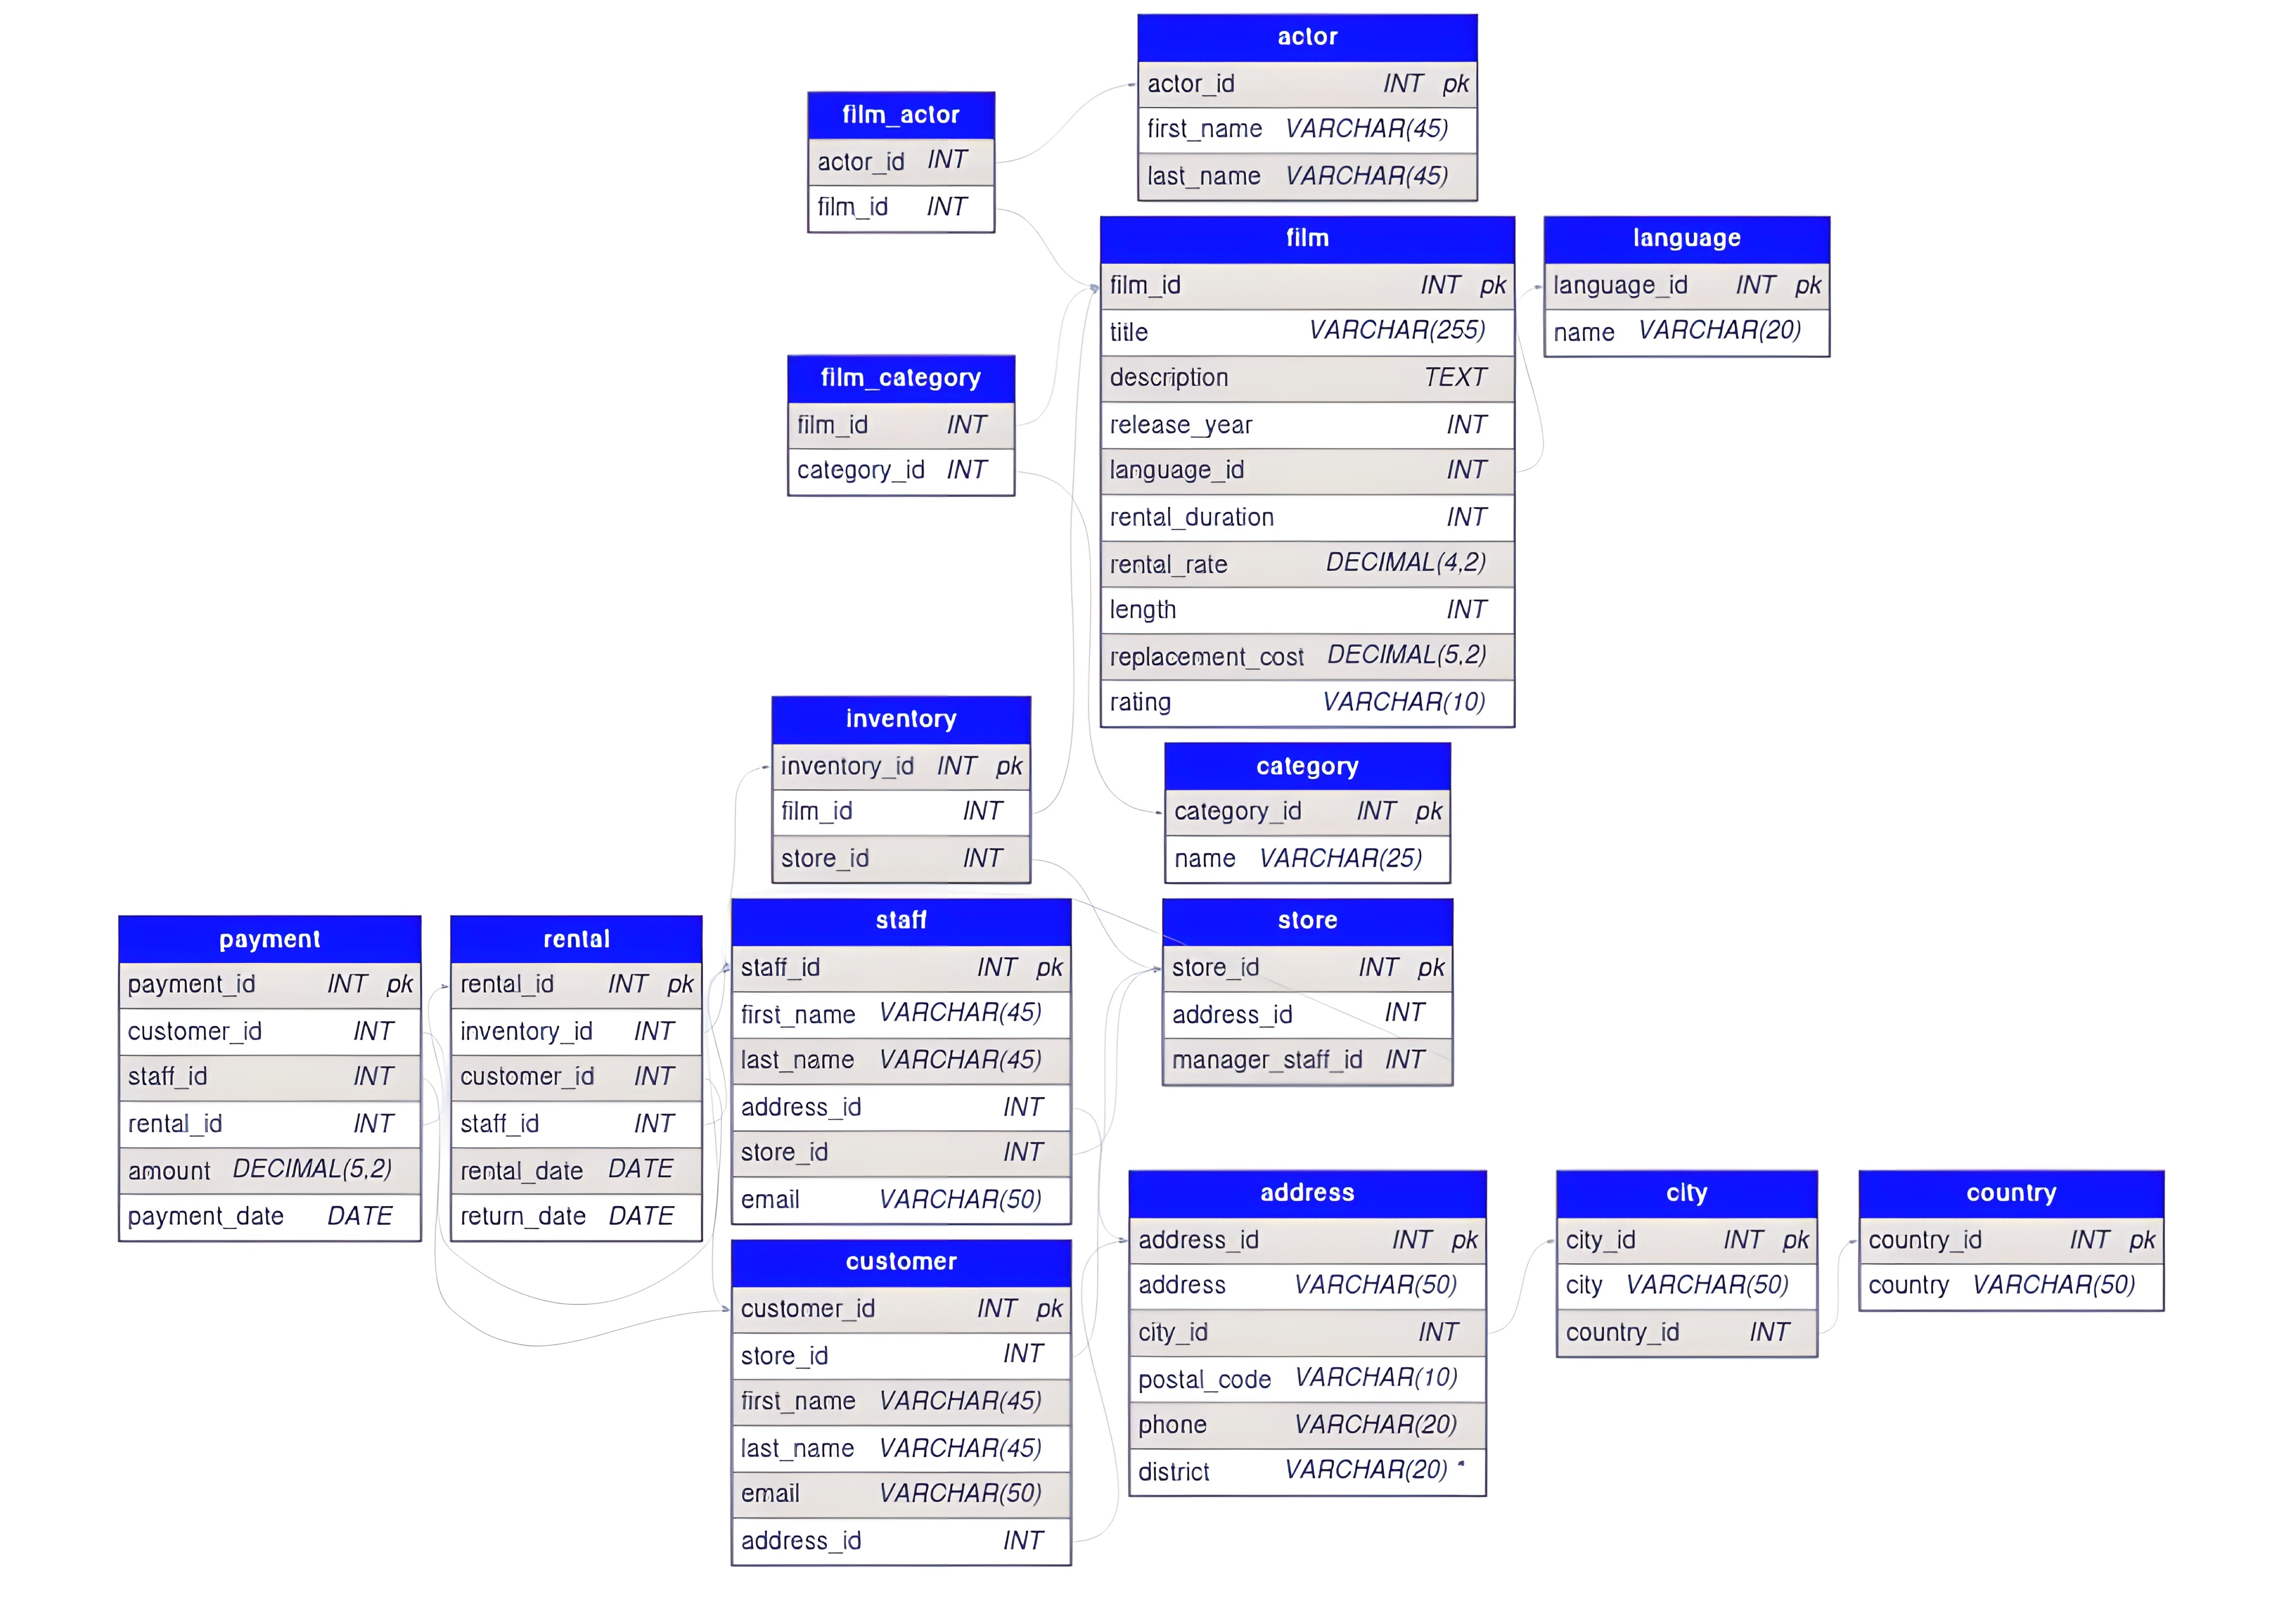
\includegraphics[width=\linewidth]{lab_08_dvdrental_1.png}
\end{figure}

\begin{enumerate}

    \item Display the titles of films that start with a vowel.

    \ifshowsolutions
    \begin{lstlisting}[language=SQL]
    SELECT title
    FROM film
    WHERE LOWER(title) LIKE 'a%'
       OR LOWER(title) LIKE 'e%'
       OR LOWER(title) LIKE 'i%'
       OR LOWER(title) LIKE 'o%'
       OR LOWER(title) LIKE 'u%';
    \end{lstlisting}
    \fi
        
    \item List all distinct film ratings available in the database.

    \ifshowsolutions
    \begin{lstlisting}[language=SQL]
    SELECT DISTINCT rating
    FROM film;
    \end{lstlisting}
    \fi
    

    \item Display the ID, first and last name for customers who have rented films from every store in the database.

    \ifshowsolutions
    \begin{lstlisting}[language=SQL]
    SELECT c.customer_id, c.first_name, c.last_name
    FROM customer c
    JOIN rental r ON c.customer_id = r.customer_id
    JOIN inventory i ON r.inventory_id = i.inventory_id
    GROUP BY c.customer_id, c.first_name, c.last_name
    HAVING COUNT(DISTINCT i.store_id) = (SELECT COUNT(*) FROM store);
    \end{lstlisting}
    \fi
    


    \item Identify customers who rented films in at least two different months.

    \ifshowsolutions
    \begin{lstlisting}[language=SQL]
    SELECT customer_id
    FROM rental
    GROUP BY customer_id
    HAVING COUNT(DISTINCT EXTRACT(MONTH FROM rental_date)) >= 2;
    \end{lstlisting}
    \fi


    \item Find the total number of rentals handled by each staff member. Display staff name and rental count.
    
    \ifshowsolutions
    \begin{lstlisting}[language=SQL]
    SELECT s.first_name, s.last_name, COUNT(r.rental_id) AS rental_count
    FROM staff s
    JOIN rental r ON s.staff_id = r.staff_id
    GROUP BY s.staff_id, s.first_name, s.last_name;
    \end{lstlisting}
    \fi



        \item Find films whose rental duration is longer than 5 days.

    \ifshowsolutions
    \begin{lstlisting}[language=SQL]
    SELECT title, rental_duration
    FROM film
    WHERE rental_duration > 5;
    \end{lstlisting}
    \fi


    \item Show the total number of films available in each category.

    \ifshowsolutions
    \begin{lstlisting}[language=SQL]
    SELECT ca.name AS category, COUNT(fc.film_id) AS film_count
    FROM category ca
    JOIN film_category fc ON ca.category_id = fc.category_id
    GROUP BY ca.category_id, ca.name;
    \end{lstlisting}
    \fi
    
    
    \item Find customers whose average rental duration is greater than 3 days.

    \ifshowsolutions
    \begin{lstlisting}[language=SQL]
    SELECT c.customer_id, c.first_name, c.last_name
    FROM customer c
    JOIN rental r ON c.customer_id = r.customer_id
    WHERE r.return_date IS NOT NULL
    GROUP BY c.customer_id, c.first_name, c.last_name
    HAVING AVG(EXTRACT(DAY FROM (r.return_date - r.rental_date))) > 3;
    \end{lstlisting}
    \fi



    
    \item Find customers who have rented films from every category available in the database.

    \ifshowsolutions
    \begin{lstlisting}[language=SQL]
    SELECT c.customer_id, c.first_name, c.last_name
    FROM customer c
    JOIN rental r ON c.customer_id = r.customer_id
    JOIN inventory i ON r.inventory_id = i.inventory_id
    JOIN film_category fc ON i.film_id = fc.film_id
    GROUP BY c.customer_id, c.first_name, c.last_name
    HAVING COUNT(DISTINCT fc.category_id) =
           (SELECT COUNT(*) FROM category);
    \end{lstlisting}
    \fi


    \item For each category, list the actor(s) who appeared in the most films in that category. 
    \ifshowsolutions
    \begin{lstlisting}[language=SQL]
    SELECT 
        c.name AS category_name, 
        a.first_name, 
        a.last_name, 
        COUNT(*) AS film_count
    FROM film_category fc
    JOIN film_actor fa ON fc.film_id = fa.film_id
    JOIN actor a ON fa.actor_id = a.actor_id
    JOIN category c ON fc.category_id = c.category_id
    GROUP BY c.category_id, c.name, a.actor_id, a.first_name, a.last_name
    HAVING COUNT(*) = (
        SELECT MAX(actor_film_count)
        FROM (
            SELECT fa2.actor_id, COUNT(*) AS actor_film_count
            FROM film_category fc2
            JOIN film_actor fa2 ON fc2.film_id = fa2.film_id
            WHERE fc2.category_id = c.category_id
            GROUP BY fa2.actor_id
        ) AS sub
    );
    \end{lstlisting}
    \fi

\end{enumerate}

\end{document}
